% Created 2017-07-14 Fri 20:50
% Intended LaTeX compiler: pdflatex
\documentclass[11pt]{article}
\usepackage[utf8]{inputenc}
\usepackage[T1]{fontenc}
\usepackage{graphicx}
\usepackage{grffile}
\usepackage{longtable}
\usepackage{wrapfig}
\usepackage{rotating}
\usepackage[normalem]{ulem}
\usepackage{amsmath}
\usepackage{textcomp}
\usepackage{amssymb}
\usepackage{capt-of}
\usepackage{hyperref}
\author{Francesco Antonello Ferraro}
\date{\today}
\title{Trabalho T2}
\hypersetup{
 pdfauthor={Francesco Antonello Ferraro},
 pdftitle={Trabalho T2},
 pdfkeywords={},
 pdfsubject={},
 pdfcreator={Emacs 25.2.1 (Org mode 9.0.7)}, 
 pdflang={English}}
\begin{document}

\maketitle
\newpage

\section{Esquema}
\label{sec:org301df5d}

O esquema não foi modificado. Permaneceu o mesmo do trabalho 1.


\begin{verbatim}
CREATE TABLE FUNCIONARIO (
    MATRICULA NUMBER(9),
    SENHA VARCHAR(20),
    NASCIMENTO DATE,
    DATA_ADMISSAO DATE,
    SEXO VARCHAR(1),
    NOME VARCHAR(35),
    ENDERECO VARCHAR(35),
    SALARIO NUMBER(5),
    PRIMARY KEY (MATRICULA)
);

CREATE TABLE EQUIPAMENTO (
    IDENTIFICADOR NUMBER(9),
    DATA_AQUISICAO DATE,
    DESCRICAO VARCHAR(100),
    CUSTO_DIARIA NUMBER(10),
    PRIMARY KEY (IDENTIFICADOR)
);

CREATE TABLE RESERVAS(
    MATRICULA NUMBER(9),
    IDENTIFICADOR NUMBER(9),
    PROTOCOLO INT,
    DATA_INICIO DATE,
    DATA_TERMINO DATE,
    PRIMARY KEY (PROTOCOLO),
    CONSTRAINT FK_MATRICULA 
    	       FOREIGN KEY (MATRICULA) 
	       REFERENCES FUNCIONARIO (MATRICULA),
    CONSTRAINT FK_IDENTIFICADOR
    	       FOREIGN KEY (IDENTIFICADOR)
	       REFERENCES EQUIPAMENTO (IDENTIFICADOR)
);
\end{verbatim}
\section{Programa}
\label{sec:org54218c6}

Para rodar o trabalho, o usuário deve entrar na pasta e rodar o seguinte comando:

\begin{itemize}
\item \emph{./gradlew run}
\end{itemize}

O programa traz um menus com as possíveis ações que o usuário pode
emitir, assim como demostrado na figura abaixo.

\begin{center}
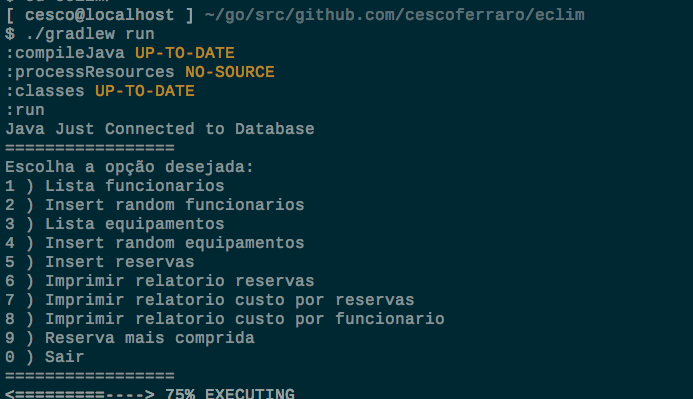
\includegraphics[width=.9\linewidth]{./static/menu.png}
\end{center}

\subsection{Comandos}
\label{sec:org09b0108}
\subsubsection{Lista Funcionários}
\label{sec:orgd98e27b}
Exibe uma lista com todos os funcionários presentes na database.
\subsubsection{Insert Random Funcionários}
\label{sec:org12d99af}
Insere um funcionário na database com informações aleatórias. 
Imprime o número da matrícula do funcionário inserido.
\subsubsection{Lista Equipamentos}
\label{sec:org0ba8dfa}
Exibe uma lista com todos os equipamentos presentes na database.
\subsubsection{Insert Random Equipamentos}
\label{sec:org92765fc}
Insere um equipamento na database com informações aleatórias. 
Imprime o identificador do equipamento inserido.
\subsubsection{Insert Reservas}
\label{sec:org384ee2e}
Insere um reserva na database. Perguntando qual a matricula do
funcionário que vai realizar a reserva e o identificador do
equipamento que vai ser reservado.
\begin{center}
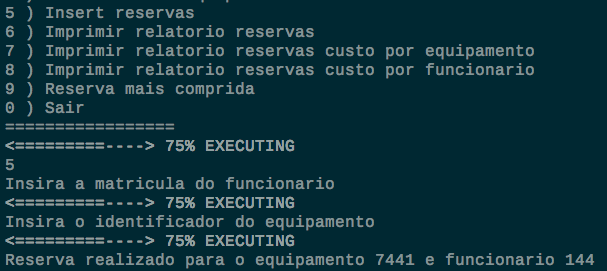
\includegraphics[width=.9\linewidth]{./static/reservas.png}
\end{center}
\subsubsection{Imprimir Relatório Reservas}
\label{sec:orga8fb190}
Lista todas as reservas que ainda não começaram. 
\subsubsection{Imprimir Relatório Reservas Por Equipamento}
\label{sec:org9ba46de}
Exibe relatório sobre o custo das reservas de cada equipamento.
\subsubsection{Imprimir Relatório Reservas Por Funcionários}
\label{sec:org795b4cb}
Exibe relatório sobre o custo das reservas de cada funcionários.
\subsubsection{Reserva mais Longa}
\label{sec:org45c1ce1}
Imprime o identificador da reserva maid longa na database. 
\end{document}
